%%%%%%%%%%%%%%%%%%%%%%%%%%%%%%%%%%%%%%%%%%%%%%
%Lab report writeup based on template by Derek Hildreth
%%%%%%%%%%%%%%%%%%%%%%%%%%%%%%%%%%%%%%%%%%%%%%

\documentclass[aps,letterpaper,10pt]{article}

\usepackage{graphicx} % For images
\usepackage{float}    % For tables and other floats
\usepackage{verbatim} % For comments and other
\usepackage{amsmath}  % For math
\usepackage{amssymb}  % For more math
\usepackage{fullpage} % Set margins and place page numbers at bottom center
\usepackage{subfig}   % For subfigures
\usepackage[usenames,dvipsnames]{color} % For colors and names
\usepackage{fancyhdr} %headers
\usepackage{wrapfig} % for inline images

\usepackage{easytable}

%%%%%%%%%%%%

%HEADER FORMATING%%%%%%%%%%%%%
\pagestyle{fancy}
\headheight 23pt
\setlength{\headsep}{20pt}
\lhead{18.369 - PSet 3}
\chead{Due 11 March 2016}
\rhead{A.G. Athanassiadis}
%%%%%%%%%%%%%%%%%%%%%%%%

%Custom Definitions%%%%%%%%%%%%%%%
\newcommand{\ttt}{\texttt}
\newcommand{\D}[1]{ $D^{(#1)}$ }
%%%%%%%%%%%%%%%%%%%%%%%%

\begin{document}

\section{Problem 3}

\subsection{Part a}
\begin{figure*}[!h]
\centering
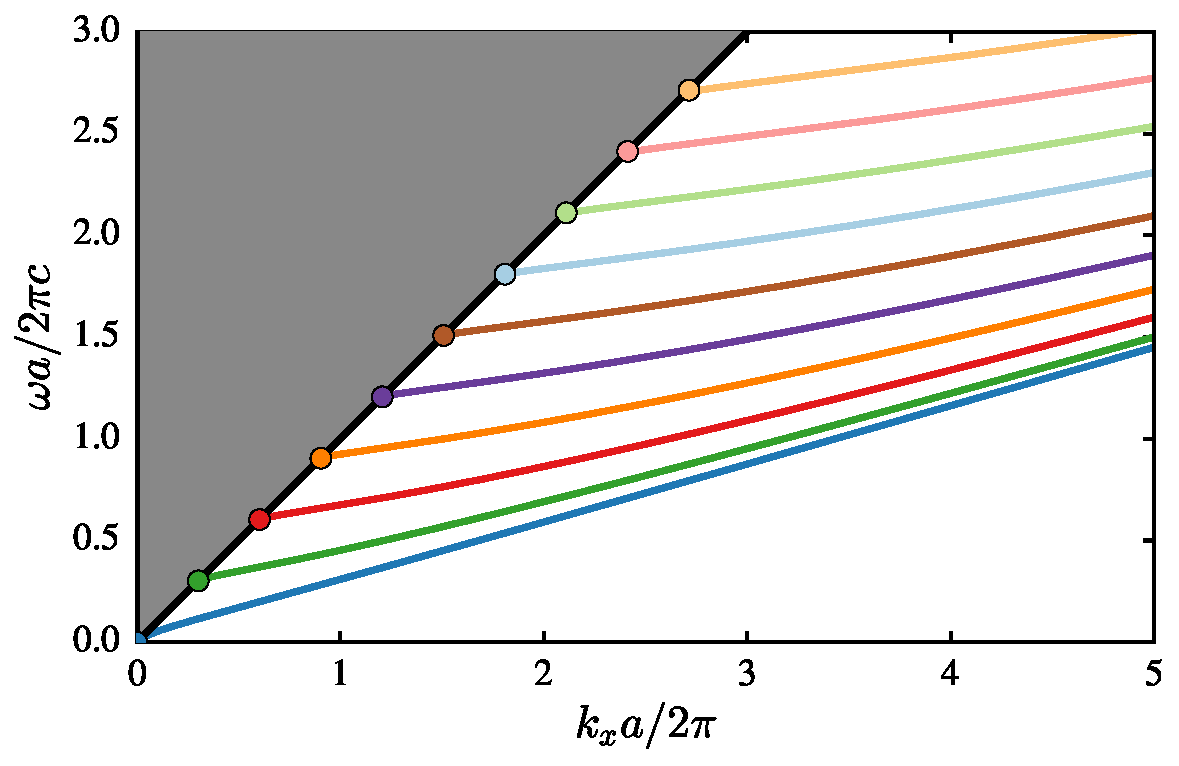
\includegraphics[width=0.6\textwidth]{3a-1}
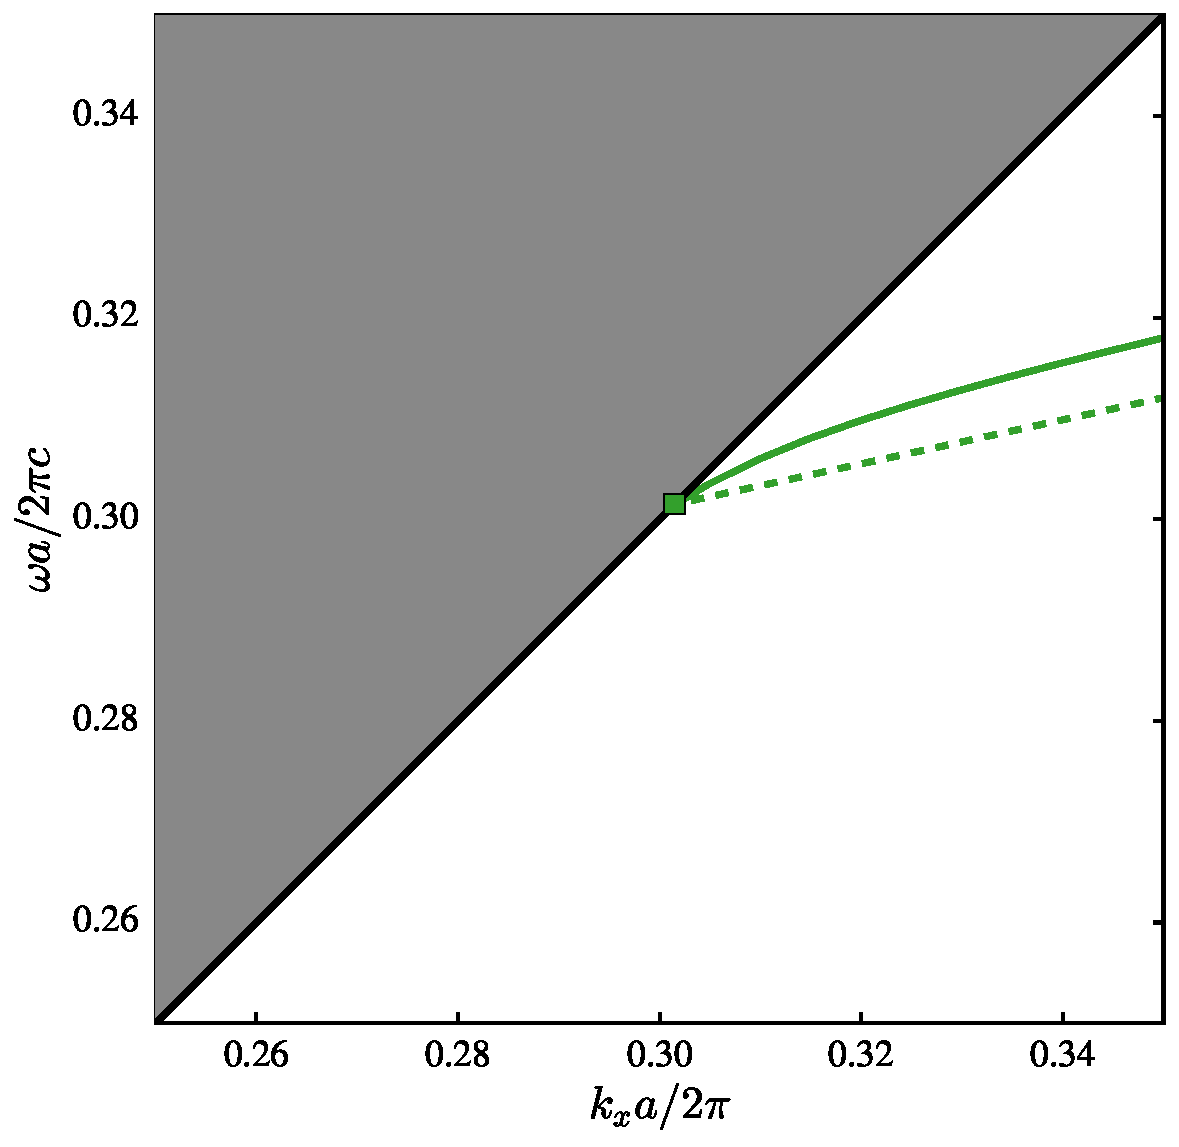
\includegraphics[width=0.39\textwidth]{3a-2}
\caption{\label{fig:3a} (left) Even mode frequency bands for the infinite waveguide. Solid markers on the light cone edge indicate the prediction for where new modes should appear. (right) Close-up of Mode 2 at low $k_x a/2\pi$. Dotted line indicates truncated computational cell (\texttt{Y=2}). As the computational cell size is increased, the the guided band $\omega(k)$ appears more tangent to the light cone. }
\end{figure*}

\subsection{Part b}
\begin{figure*}[!h]
\centering
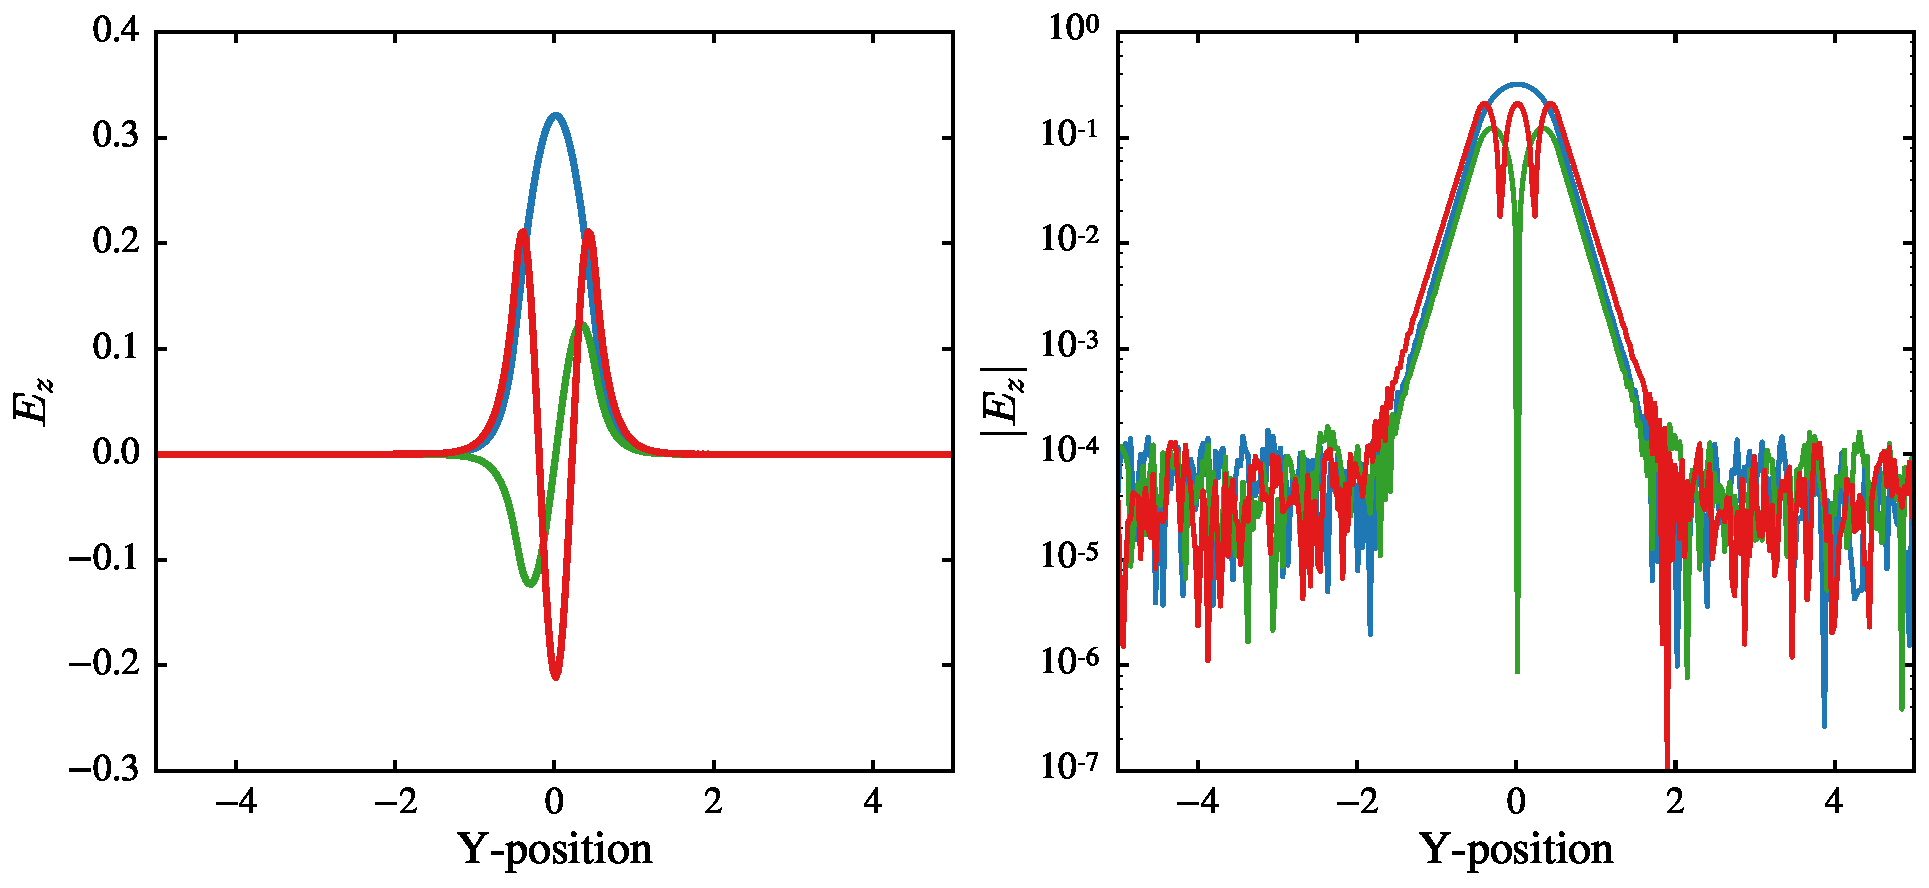
\includegraphics[width=0.9\textwidth]{3b-1}
\caption{\label{fig:3b} E-field of first 3 guided modes within the waveguide. On the right, the fields are plotted semi-log to reveal the exponential decay of the fields away from the waveguide (since it's linear on the log-scale). After decaying substantially, the field enters a noise floor around $10^{-6},$ which persists to the boundary of the computational cell.}
\end{figure*}

\subsection{Part c}
\begin{figure*}[!h]
\centering
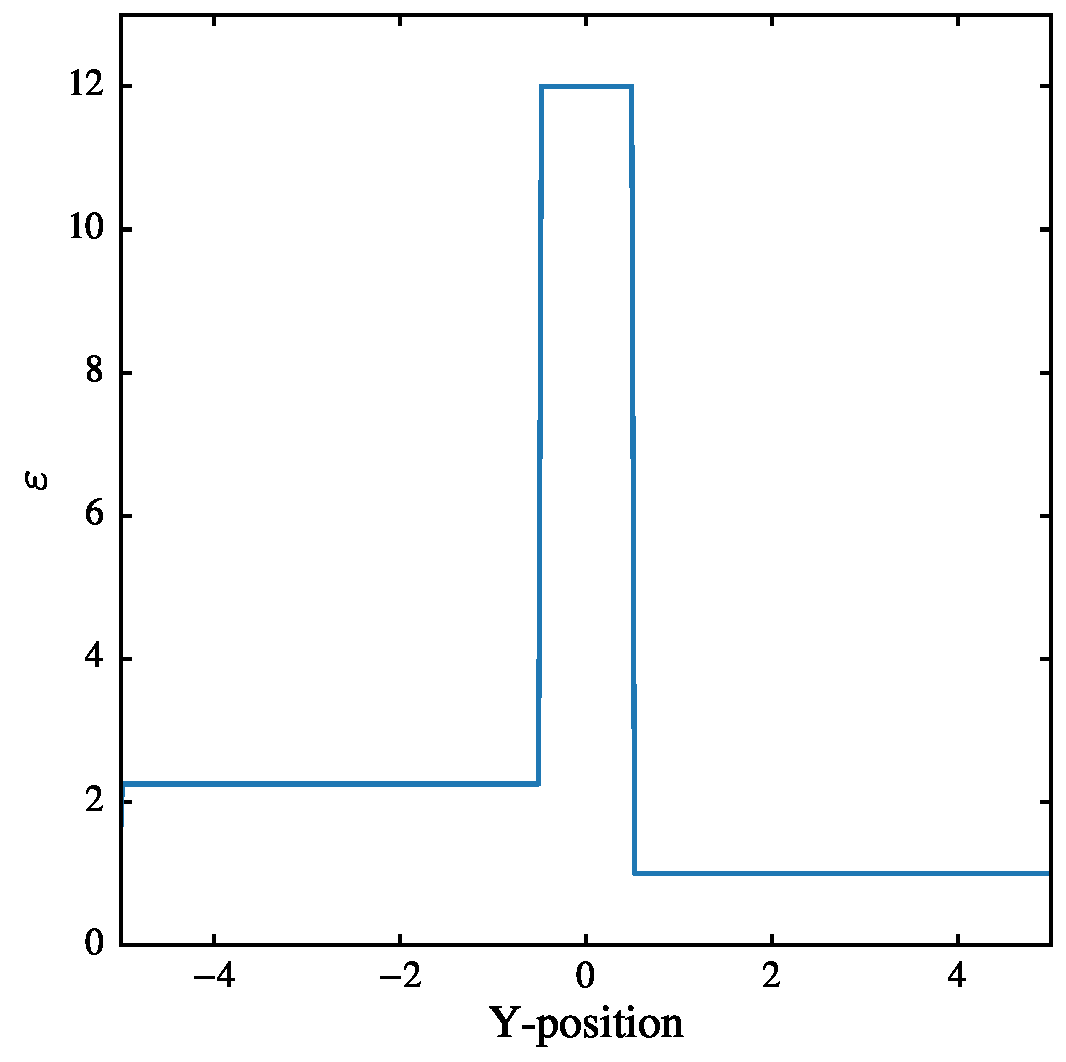
\includegraphics[width=0.3\textwidth]{3c-1}
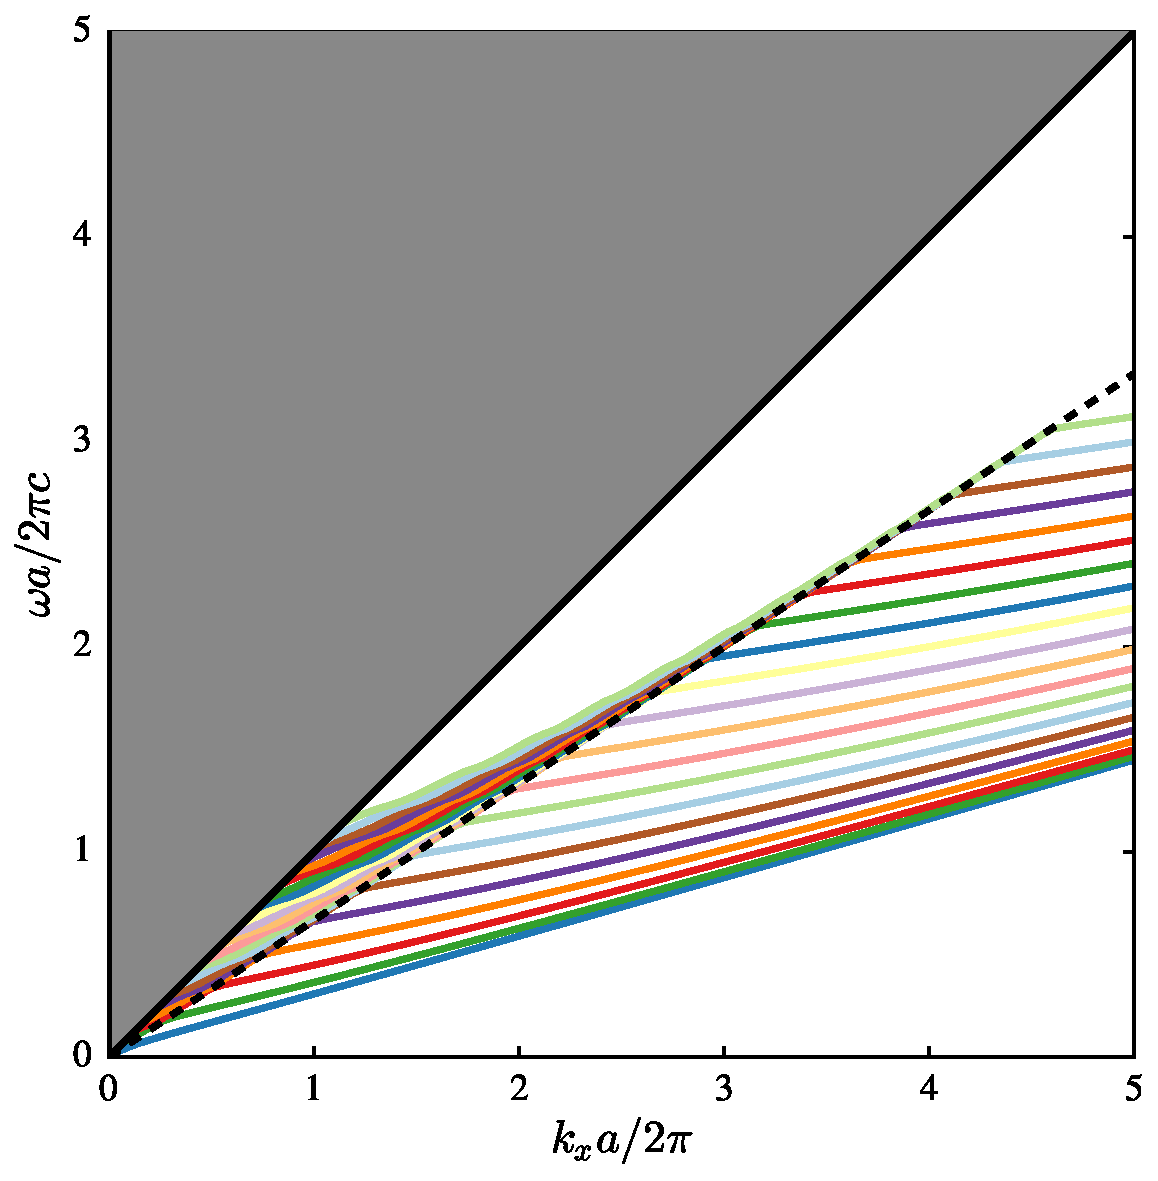
\includegraphics[width=0.3\textwidth]{3c-2}
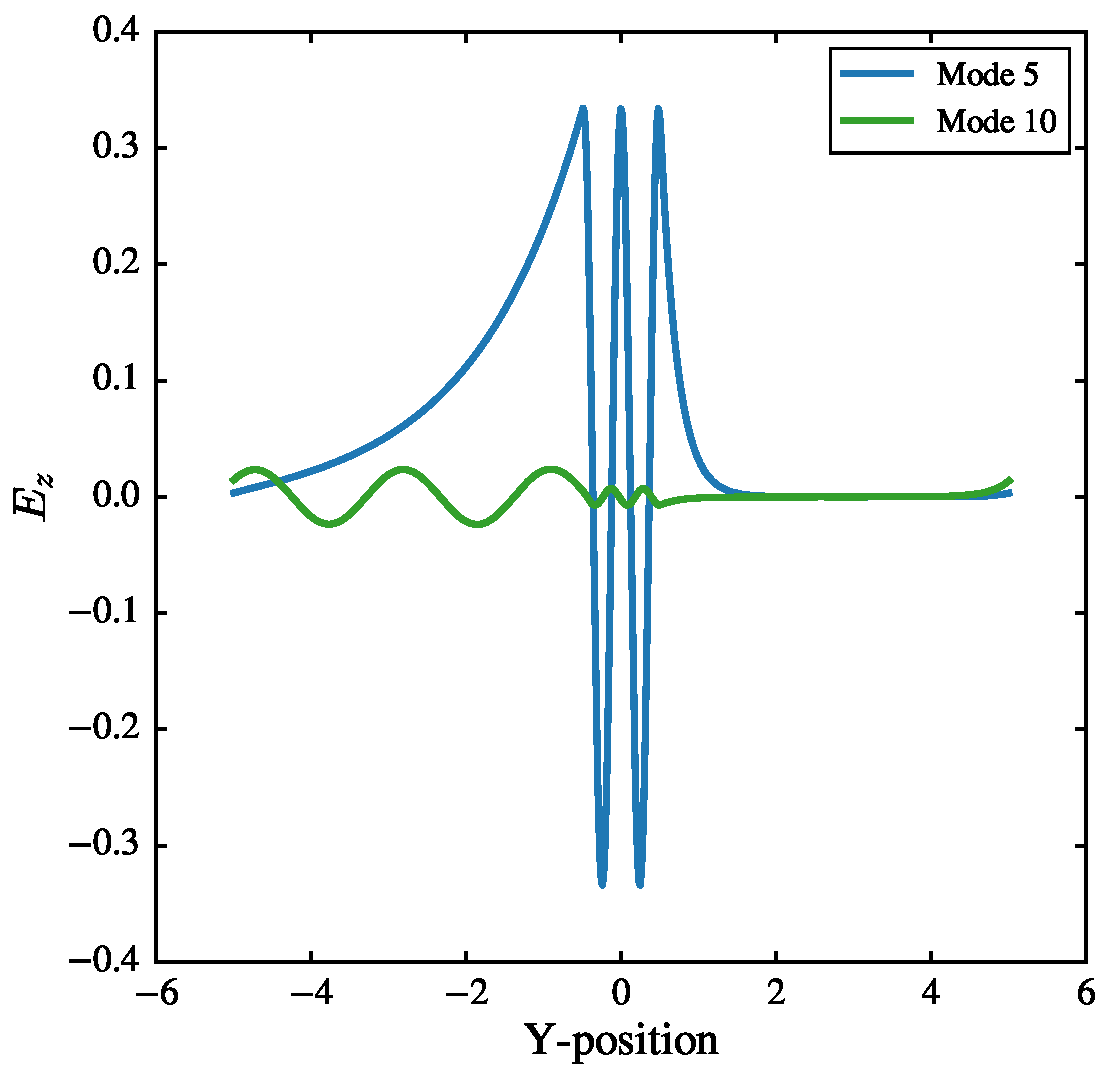
\includegraphics[width=0.3\textwidth]{3c-3}
\caption{\label{fig:3c} (Panel 1) Dielectric constant $\varepsilon$ within the computational cell. (Panel 2) The first 20 guided modes. All collapse to a new low-frequency bound below the light line. This new low-$\omega$ cutoff lies at $\omega/c = 2k_x /3$   (Panel 3) Two of the higher modes within the computational cell. The lack of symmetry in $\varepsilon$ is reflected in the asymmetric field structures that appear more clearly in higher-order modes.}
\end{figure*}


\subsection{Part d}
\begin{figure*}[!h]
\centering
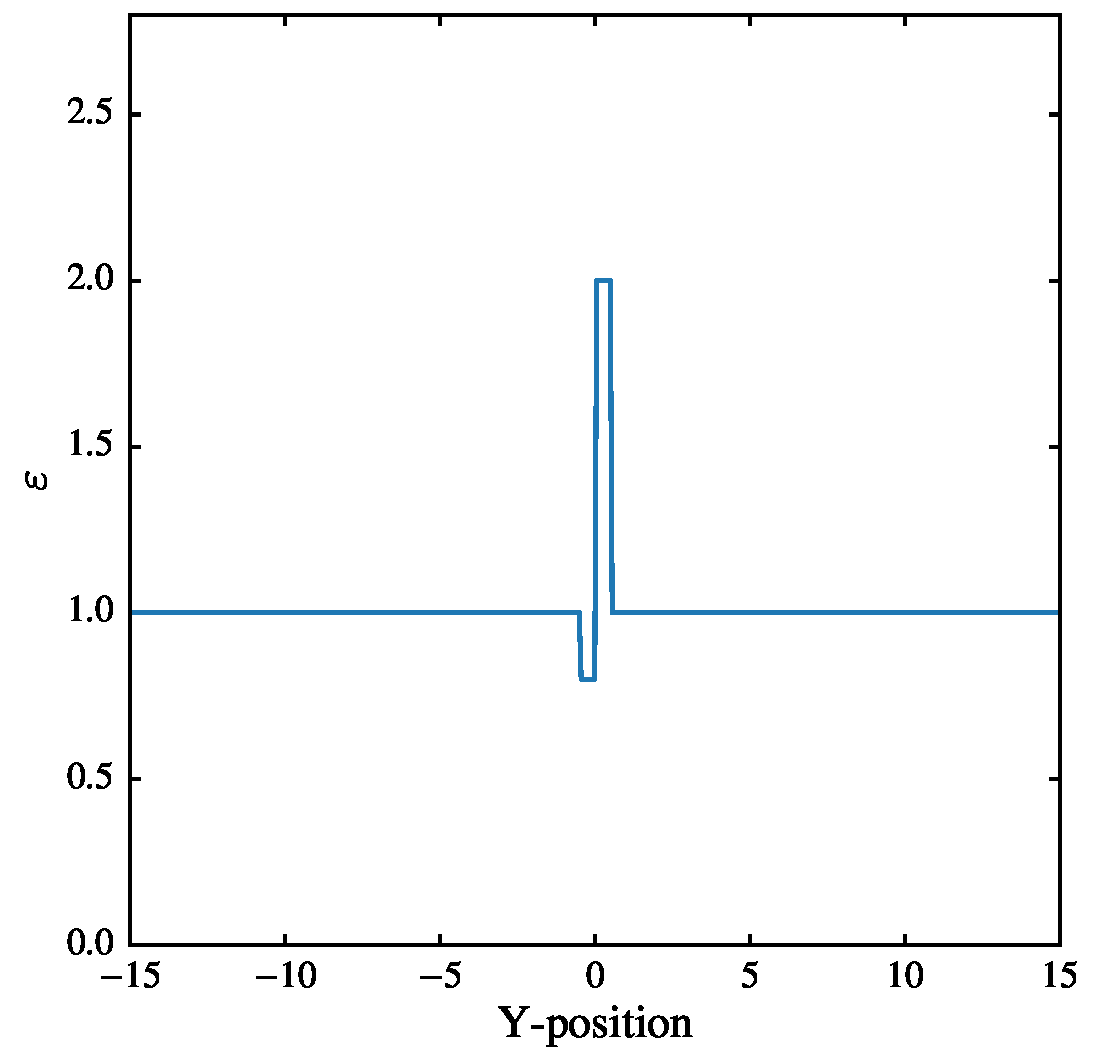
\includegraphics[width=0.3\textwidth]{3d-1}
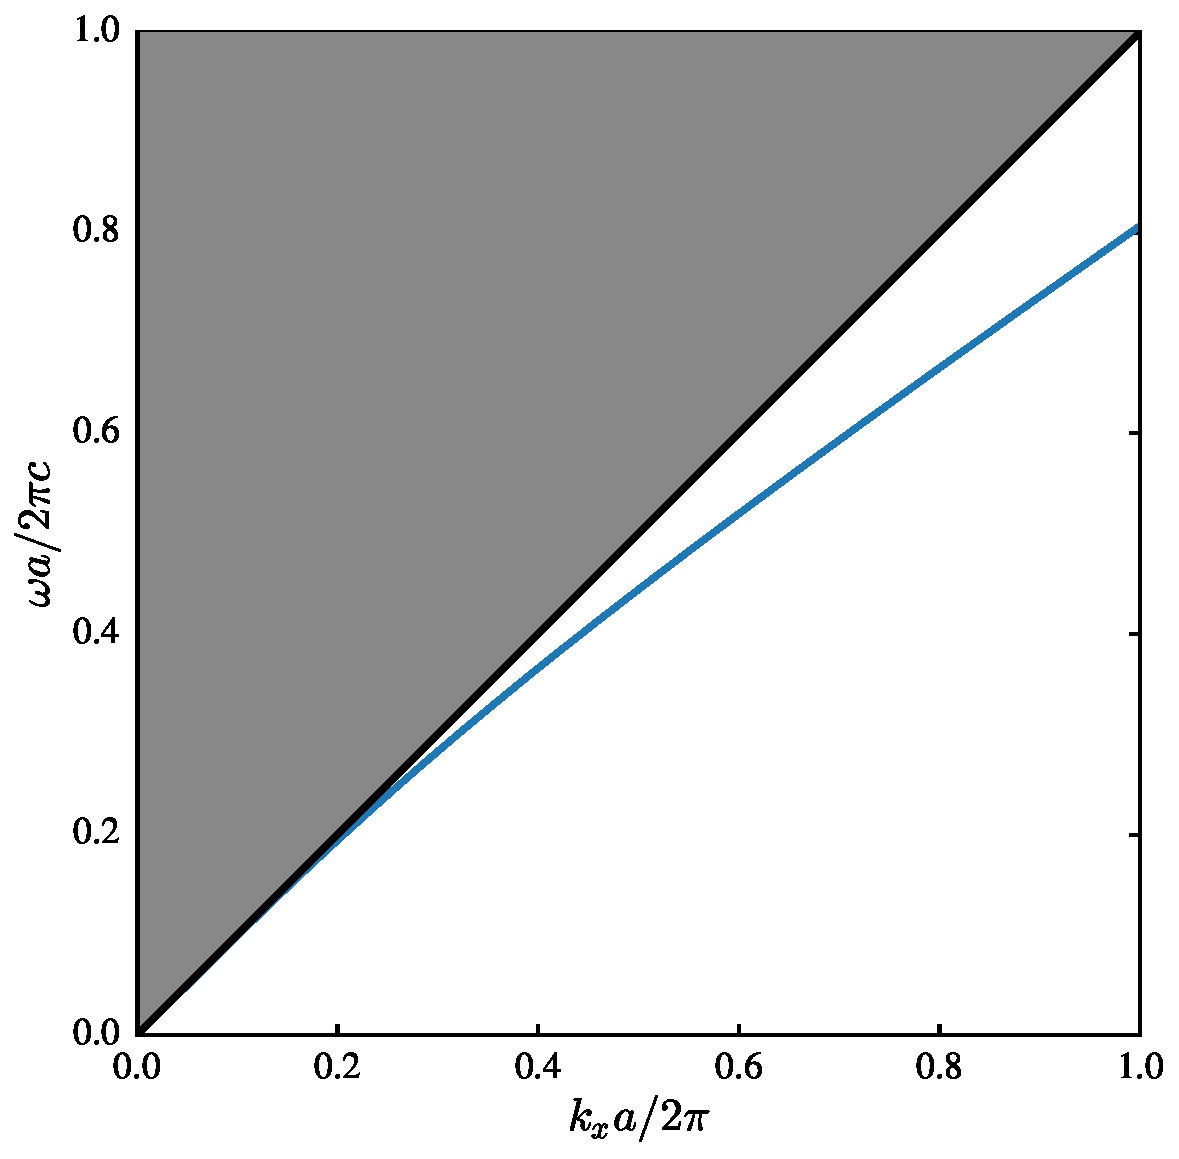
\includegraphics[width=0.3\textwidth]{3d-2}
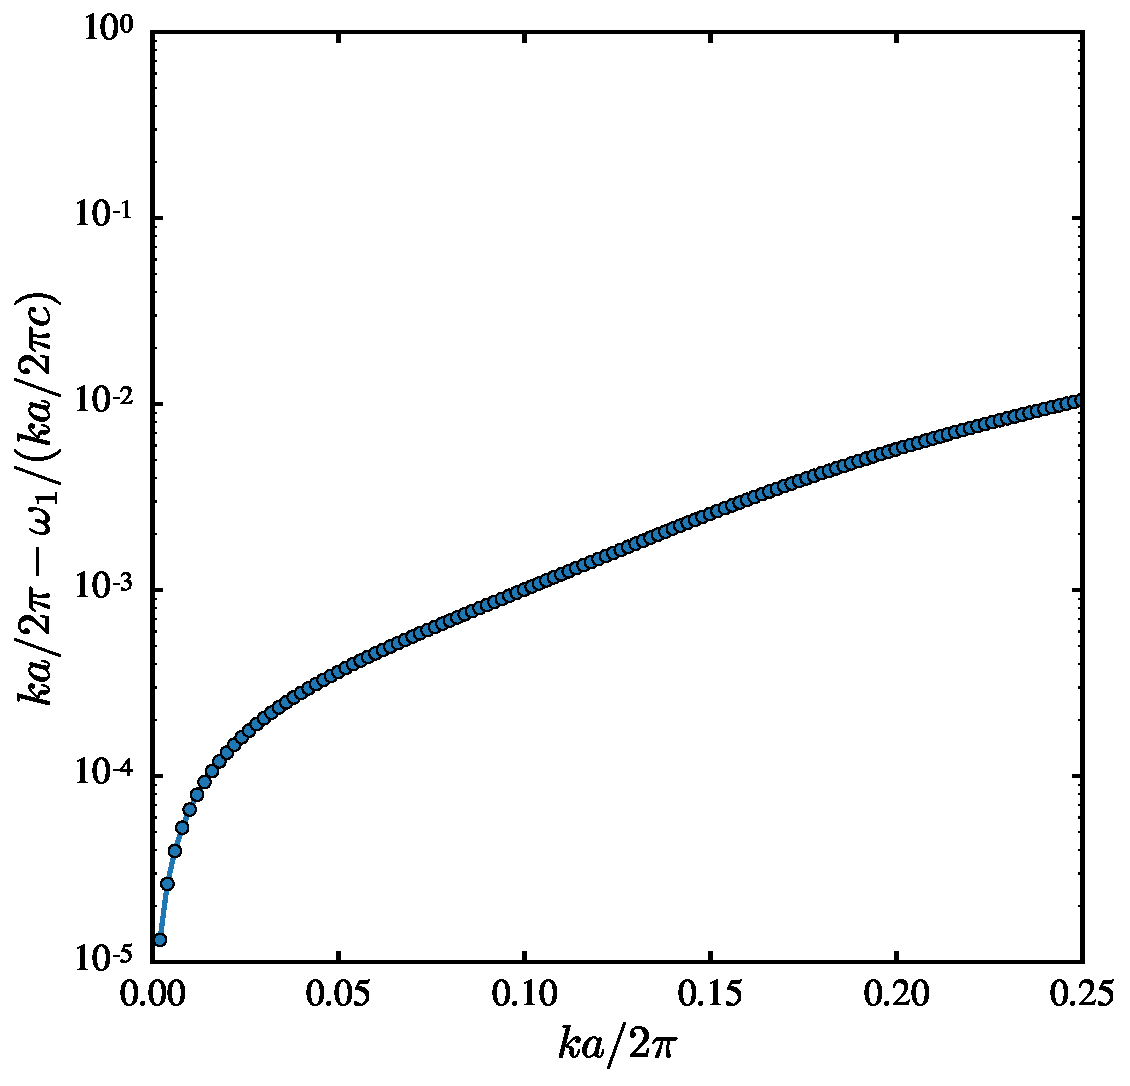
\includegraphics[width=0.3\textwidth]{3d-3}
\caption{\label{fig:3d} (Panel 1) Dielectric constant $\varepsilon$ within the computational cell. (Panel 2) First guided mode for low-$k$. This guided mode should persist to very low $k\ll a$ because as $k$ decreases, the wavelength increases and the field ``sees'' an effective medium of average dielectric constant $\varepsilon=1.4,$ which would support a guided mode. (Panel 3) Verification of this prediction - distance of the guided mode frequency from the light line. Notice how the distance is always positive, indicating that the mode persists beneath the light line (i.e. as a guided mode).}
\end{figure*}

\newpage
\section{Problem 4}
\subsection{Part a}
\begin{figure*}[!h]
\centering
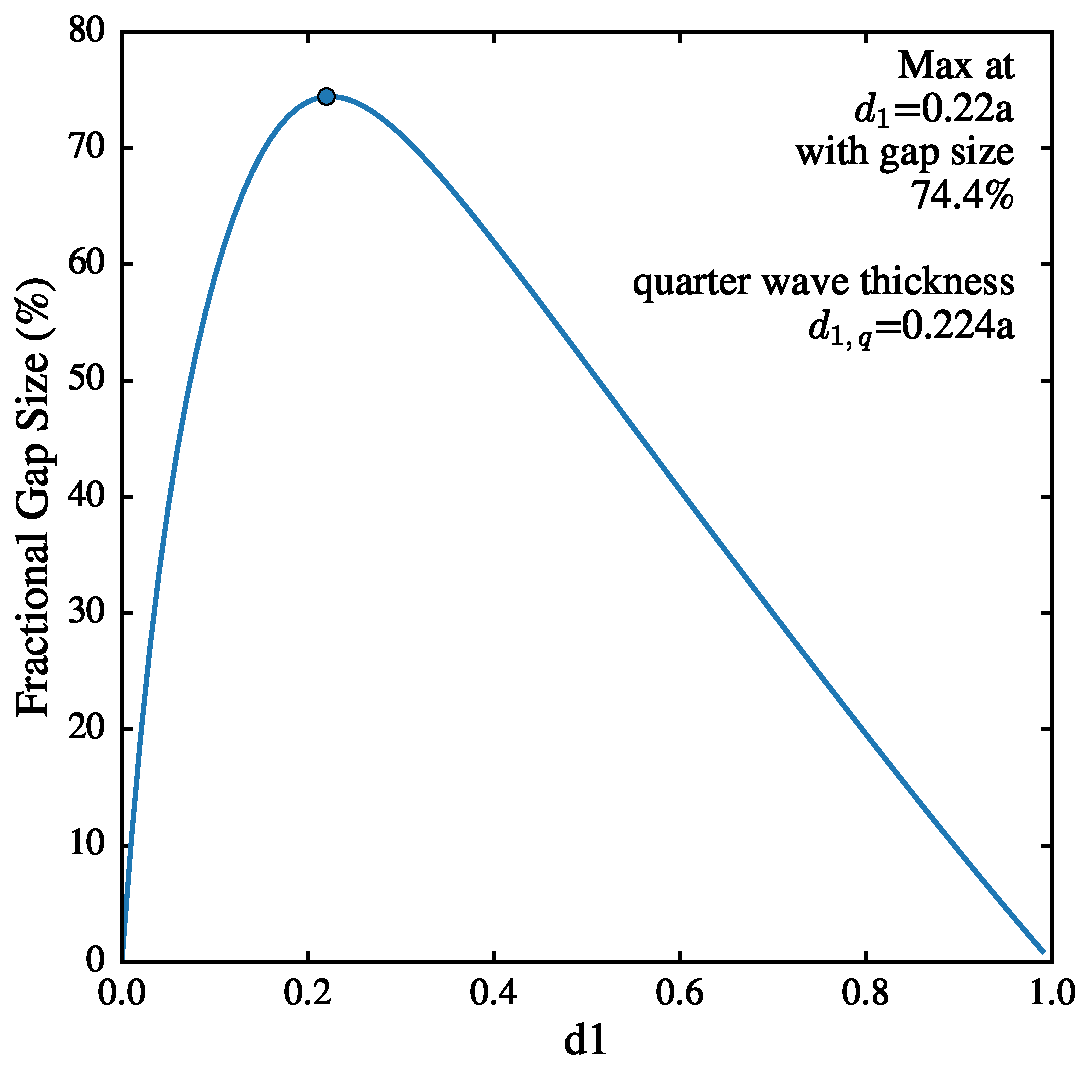
\includegraphics[width=0.4\textwidth]{4a-1}
\caption{\label{fig:4a} Fractional gap size as a function of layer 1 thickness, $d_1$. The gap size is maximized for a thickness equal to the quarter-wave thickness $d_1=d_{1,q}$.}
\end{figure*}

\subsection{Part c}
\begin{figure*}[!h]
\centering
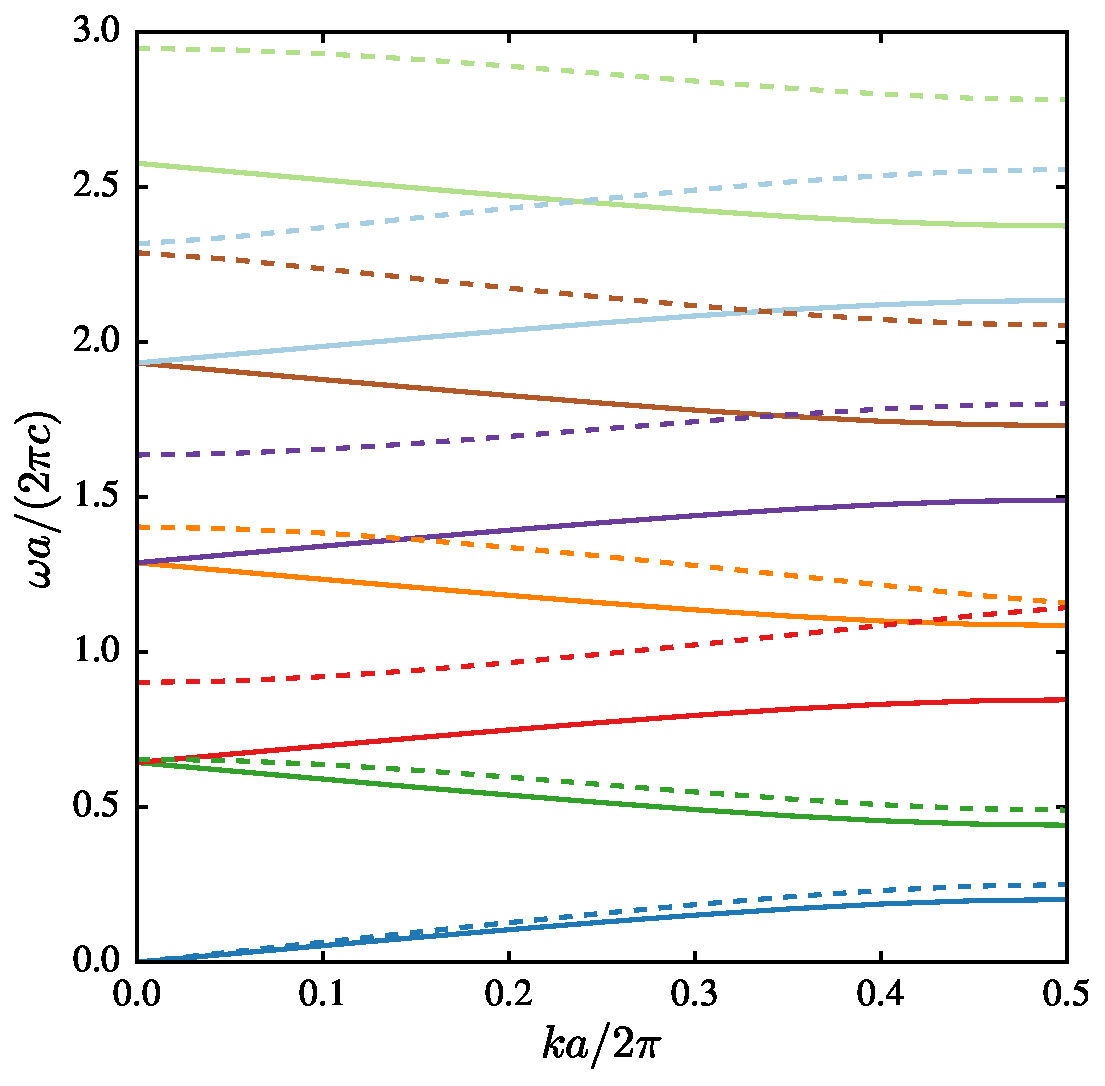
\includegraphics[width=0.5\textwidth]{4c-1}
\caption{\label{fig:4c} Band structure for $d_1 = d_{1,q}$ (solid lines) and for an arbitrary $d_1=0.12345.$ Unlike the arbitrary $d_1,$ when $d_1$ is the quarter-wave thickness, there are no gaps at $ka/2\pi=0$.}
\end{figure*}

\end{document}